\documentclass{article}

\usepackage{amsmath}
\usepackage{minted}
\usepackage{graphicx}
\graphicspath{{./images/}}

\begin{document}
    \begingroup
    % title %
    \begin{center}
        \textbf{Machine Learning Project Report}

        \vspace{1cm}

        Written by : Aung Kaung Myat
    \end{center}
    \endgroup

    \begingroup
    % Dataset Description %
    \section {Dataset Description}

    The dataset is about the usage behavior of about 9000 active credit card holders during last 6 months.
    The dataset is created based on customer level with 17 behavioral variables. 
    The dataset has 8950 observations and 18 features. 
    \endgroup

    \hfill

    \begingroup
    % Goal of the project %
    \section {Goal of the project}

    The goal of this project is to segment the credit card holders into different groups based on their usage behavior to create a marketing stragegy.
    For the new marketing strategy, the credit card holders will be grouped into at least 4 groups and not more than 10 groupus in order to be effective.
    In order to achieve the goal, clustering algorithm will be used to segment the credit card holders into different groups.
    \endgroup

    \hfill

    \begingroup
    % Data Exploration%
    \section {Data Exploration}
    
    The dataset contains 18 features and 8950 observations.
    There is one categorical feature and 17 numerical features.
    The categorical feature is CUST\_ID. As it does not have useful information about behavior of the credit card holders, it will be dropped.
    The numerical features are BALANCE, BALANCE\_FREQUENCY, PURCHASES, ONEOFF\_PURCHASES, INSTALLMENTS\_PURCHASES, CASH\_ADVANCE, PURCHASES\_FREQUENCY, ONEOFF\_PURCHASES\_FREQUENCY, PURCHASES\_INSTALLMENTS\_FREQUENCY, CASH\_ADVANCE\_FREQUENCY, CASH\_ADVANCE\_TRX, PURCHASES\_TRX, CREDIT\_LIMIT, PAYMENTS, MINIMUM\_PAYMENTS, PRC\_FULL\_PAYMENT, TENURE.
    \hfill

    \begingroup
        \subsection{Data Visualization}

        \begin{figure}[h]
            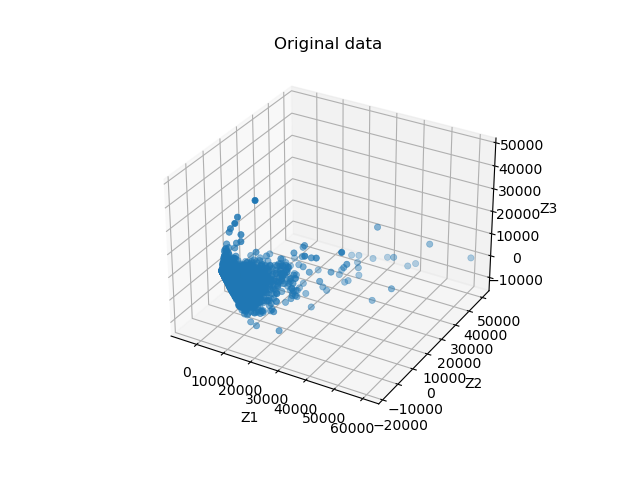
\includegraphics[scale=0.5]{original_data_vis.png}
            \caption{Original Data}
            \label{fig:original_data_vis}
        \end{figure}

        As shown in the figure \ref{fig:original_data_vis}, the data contains outliers and it is squashed to the left corner. 
        Since the data is squashed to the left corner, it is hard to see the distribution of the data.
    \endgroup

    \hfill

    \begingroup
    % Checking the missing data %
    \subsection {Checking the missing data}

    It is important to check the missing data.
    There are missing values in two features: \textit{MINIMUM\_PAYMENTS} and \textit{CREDIT\_LIMIT }.
    In \textit{MINIMUM\_PAYMENTS} there are 313 missing values and in \textit{CREDIT\_LIMIT} there are 1 missing value.
    
    \endgroup
    
    \hfill

    \begingroup
        \subsection{Checking the outliers}

        The outliers are checked using the boxplot. As can be seen in the figure \ref{fig:original_data_boxplot}, there are outliers in most of the features.

        \begin{figure}[h]
            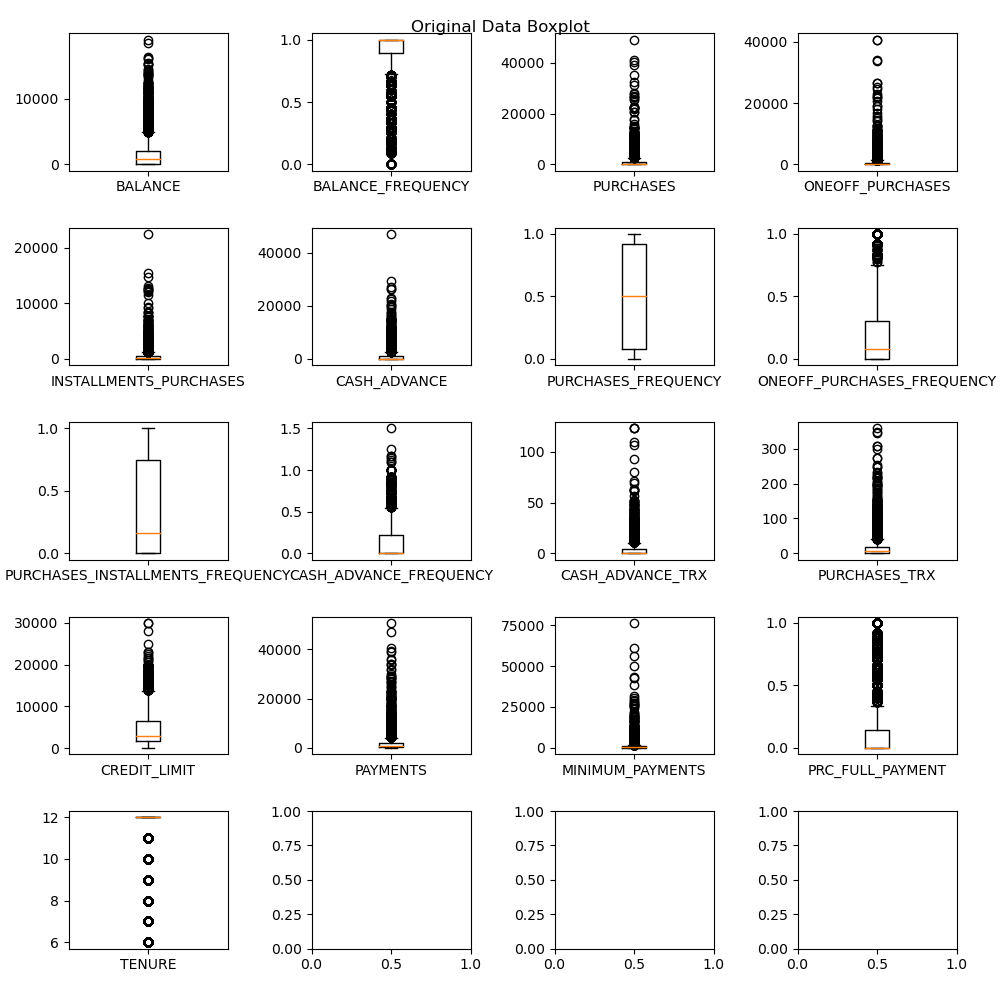
\includegraphics[scale=0.475]{original_data_boxplot.png}
            \caption{Original Data Boxplot}
            \label{fig:original_data_boxplot}
        \end{figure}
    \endgroup

    \begingroup
        \subsection {Checking the distribution of data}

        The distribution of data is checked using the histogram. 
        As can be seen in the figure \ref{fig:original_data_histogram}, the data is skewed to the left or right corners.

        \begin{figure}[h]
            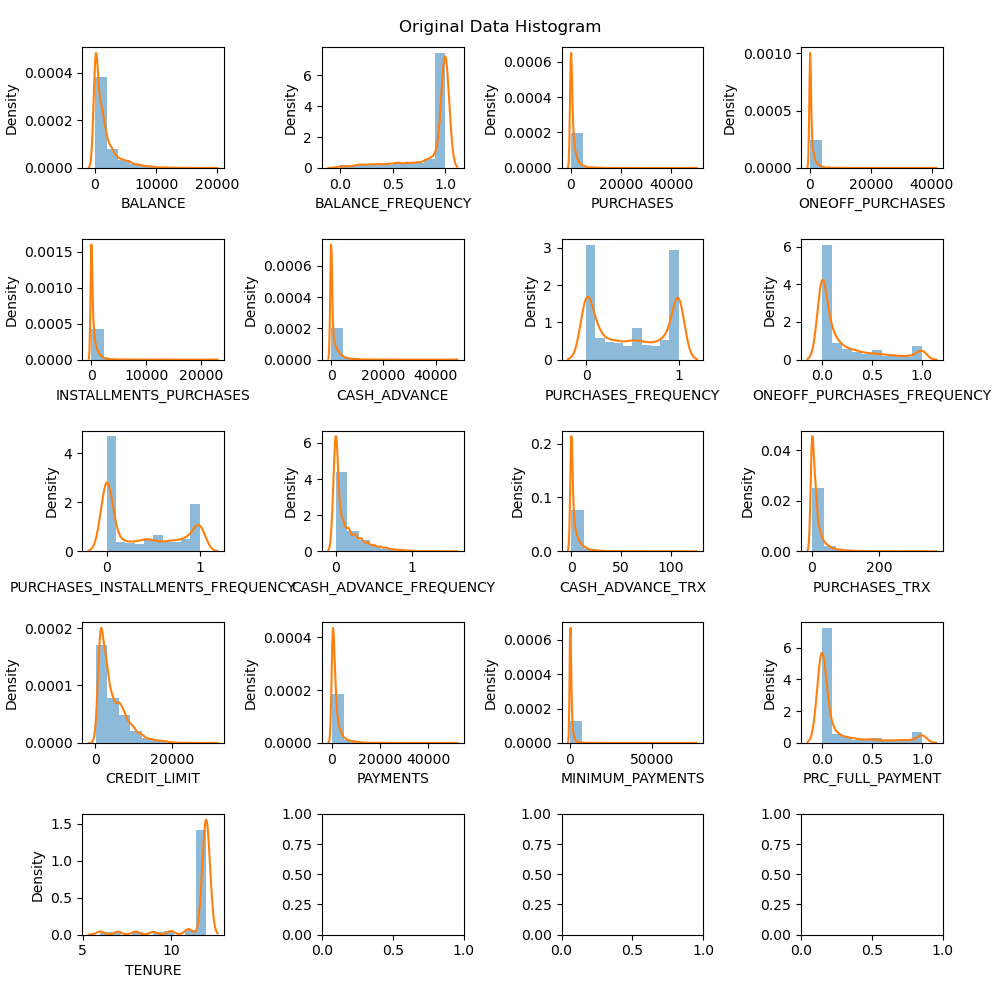
\includegraphics[scale=0.475]{original_data_histogram.png}
            \caption{Original Data Histogram}
            \label{fig:original_data_histogram}
        \end{figure}
    \endgroup

    \endgroup

    \hfill
    
    \begingroup
        \section {Data Preprocessing}
        
        \begingroup
            \subsection {Handling missing data}
            
            The missing values are handled as follows:
            \begin{itemize}
                \item Missing value in \textit{CREDIT\_LIMIT} is replaced using the mode of values because its values are not continuous values and there exisit only certain number of credit limit.
                \item Missing values of \textit{MINIMUM\_PAYMENT} is replaced with the mean of the values because its values are continuous.
            \end{itemize}
        \endgroup

        \hfill

        \begingroup
            \subsection{Handling outliers}

            The outliers are first detected using the quantile range method.
            Since the number of outliers are too many, it is not possible to remove all the outliers.
            Thus, it is better to replace with calculated values.
            In this project, 3 methods are tried for replacing the outliers values. They are:
            \begin{itemize}
                \item mean: Replacing the outliers with the mean of the values.
                \item median: Replacing the outliers with the median of the values.
                \item k-Nearest Neighbors: Replacing the outliers with the values calculated using k-nearest neighbors.
            \end{itemize}
        \endgroup

        \hfill

        \begingroup
            \subsection{Handling skewed data}

            There are many methods to handle the skewed data. 
            Two methods are tried in this project. They are:
            \begin{itemize}
                \item Logarithmic Transformation: Transforming the data using the logarithmic function.
                \item Square Root Transformation: Transforming the data using the square root function.
            \end{itemize}
        \begingroup

        \hfill

        \begingroup
            \subsection{Feature Scaling}

            Since, the scale of the features have effect on clustering algorithms, in this project normalization method is tried.
        \endgroup

        \hfill

        \begingroup
            \subsection{Dimensionality Reduction}
            
            Dimension reduction technique can filter out some noise and reduce the risk of high-dimensional datasets being very sparse.
            As a lot of noises are found in the dataset, dimensionality of the dataset is reduced using the PCA.

            The dimensionality of the dataset is reduced to 5 components.
            This is done by find the number of components that explain 95\% of the variance.

        \endgroup

        \hfill

        \begingroup
            \subsection{Data Visualization after preprocessing}

            All  the combinations of the methods are tried.
            Among them the best combination is the one that have done the following:
            \begin{itemize}
                \item outliers removal: k-Nearest Neighbors
                \item skew removel: Logarithmic Transformation
                \item scaling: no normalization
            \end{itemize}
            It can be seen on the 2nd image from the right in the 3rd row in figure \ref{fig:preprocessed_data}.
            This combination is chosen because the clusters of the data are more clearly visible.

            \begin{figure}[h]
                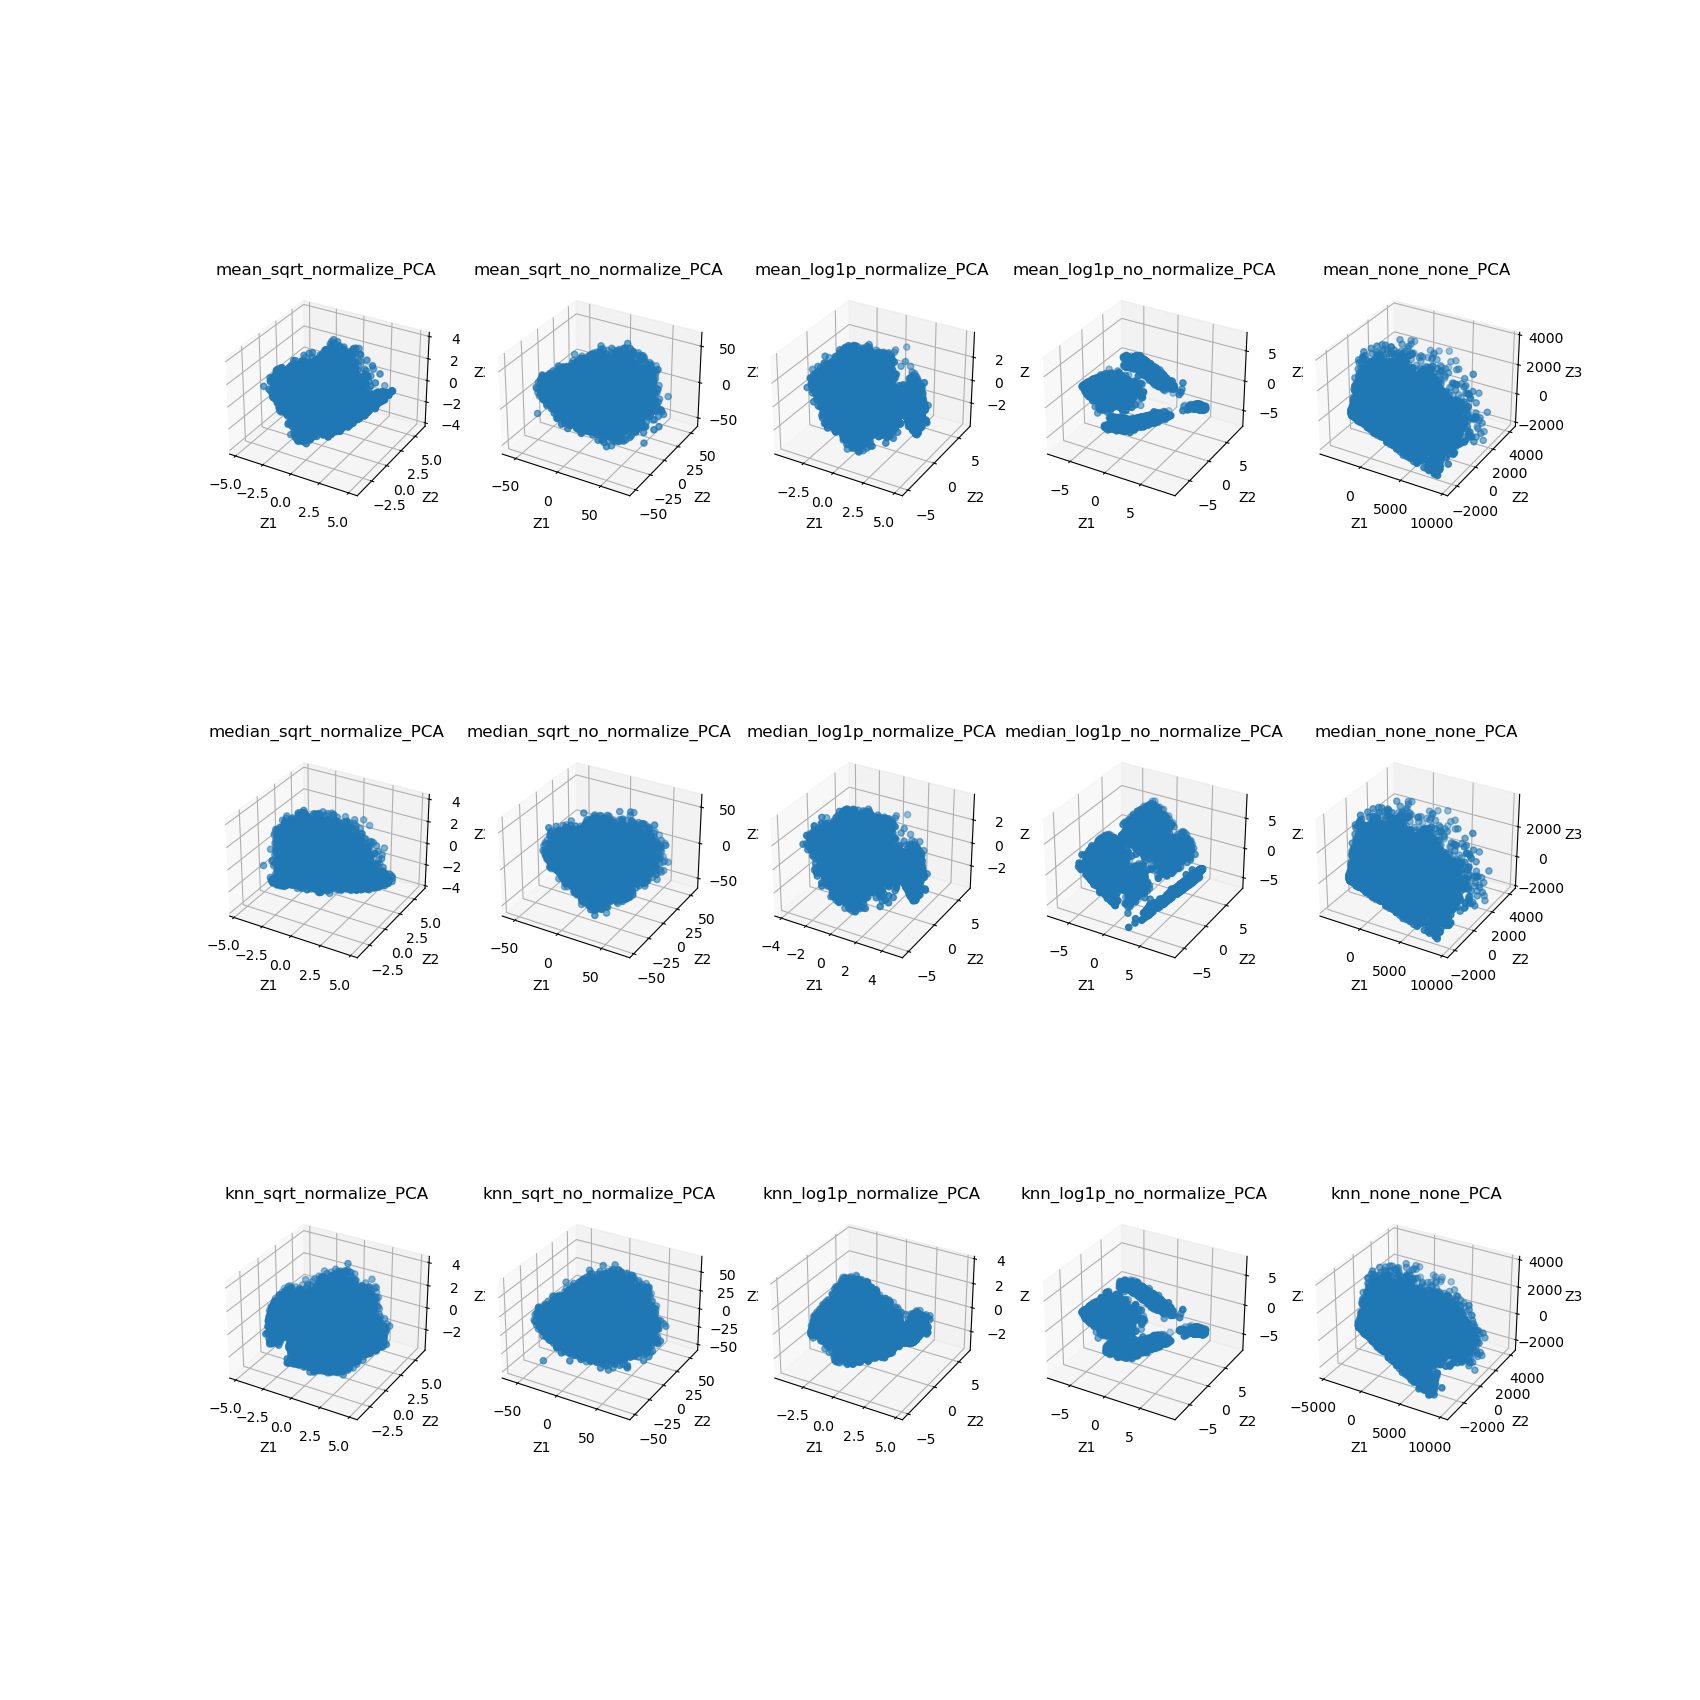
\includegraphics[scale=0.275]{data.png}
                \caption{All Combinations of the Methods}
                \label{fig:preprocessed_data}
            \end{figure}
        \endgroup

    \endgroup

    \hfill

    \begingroup
            \section{Clustering}

            To group the data into clusters, 4 clustering algorithms are tried.
            They are:
            \begin{itemize}
                \item K-Means Clustering
                \item Hierarchical Clustering
                \item DBSCAN
                \item HDBSCAN
            \end{itemize}

            \subsection{Hyperparameters}

            The hyperparameters of the algorithms are tuned using the grid search method.
            The best number of cluster is found using the silhouette score.

            The hyperparameters of the algorithms are:

            \begin{tabular}{|c|c|c|}
                \hline
                Algorithm & Hyperparameter & Value \\
                \hline
                K-Means Clustering & number of clusters & 2 to 21 \\
                \hline
                Hierarchical Clustering & number of clusters & 2 to 21 \\
                \hline
                DBSCAN & mininum points  & 5, 10, 20, 50, 100, 200  \\
                \hline
                HDBSCAN & mininum cluster size  & 5, 10, 20, 50, 100, 200  \\
                \hline
            \end{tabular}

            \hfill

            Best parameters of the algorithms are:

                \begin{tabular}{|c|c|c|c|}
                    \hline
                    Algorithm & Number of Clusters Created & Hyperparameter & Value \\
                    \hline
                    K-Means Inertia Method & 6 & number of clusters & 6 \\
                    \hline
                    K-Means Silhouette Method & 7 & number of clusters & 7 \\
                    \hline
                    Hierarchical Silhouette Method & 7 & number of clusters & 7 \\
                    \hline
                    DBSCAN Silhouette Method & 7 & mininum points  & 100  \\
                    \hline
                    HDBSCAN Silhouette Method & 10 & mininum cluster size  & 20 \\
                    \hline
                \end{tabular}

    \endgroup

    \hfill

    \begingroup
            \section{Results}

            Among the algorithms K-Means Clustering is best suited for this dataset. 
            It achieves the highest silhouette score of 0.5.
            The silhouette score of the other algorithms are 0.49 for Hierarchical Clustering, 0.48 for HDBSCAN and 0.47 for DBSCAN.
            DBSCAN performs the worst among the algorithms and many of the data are grouped as outliers. 

            In terms of data interpretability, K-Means Clustering is also the best algorithm.
            Especially, the clusters created by K-Means Clustering with inertia method gives results that have good interpretability.

            
            \begin{figure}[h]
                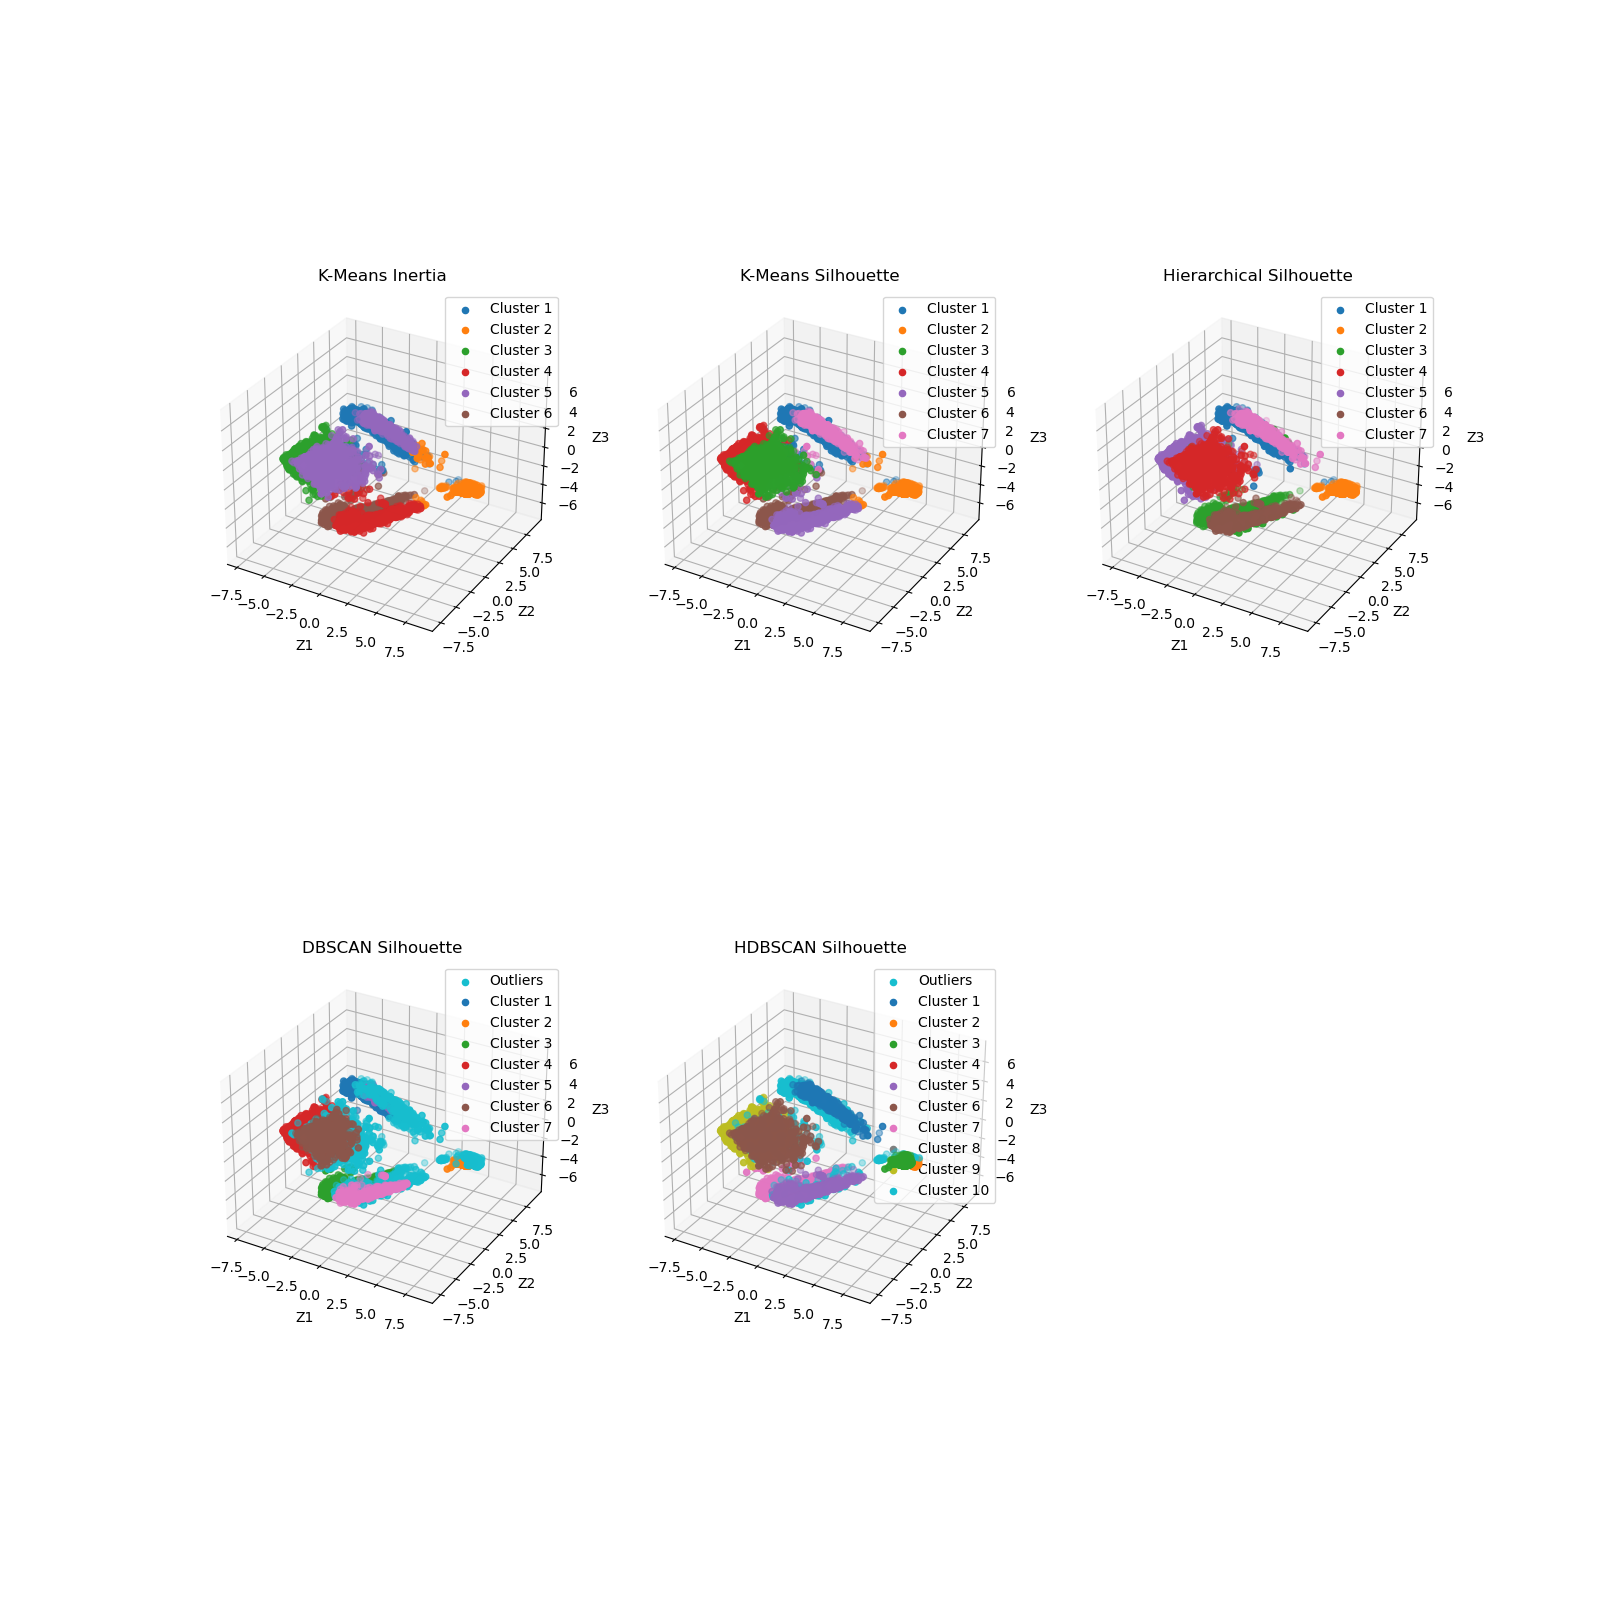
\includegraphics[scale=0.285]{clusters.png}
                \caption{Clusters According to Algorithms}
                \label{fig:clusters}
            \end{figure}

            \subsection {Interpretation of the Clusters Created by K-Means Clustering with Inertia Method}
            
            The following are the clusters created by K-Means Clustering with inertia method.

            \textbf{Cluster 1}

            This cluster contains the card holders who have the medium credit limit and do frequently intallment purchases.

            \begin{tabular}{|c|c|c|c|c|c|c|}
                \hline
                Feature & Cluster 1 & Cluster 2 & Cluster 3 & Cluster 4 & Cluster 5 & Cluster 6 \\
                \hline
                P\_INSTALLMENTS\_FREQ mean & 0.6645 & 0.0021 & 0.6535 & 0.0029	& 0.6381	& 0.0030 \\
                \hline
                CREDIT\_LIMIT min & 300 & 50	& 300 & 300 & 300 & 150 \\
                CREDIT\_LIMIT max & 23000	& 19000	& 30000	& 20000	& 30000	& 25000 \\
                \hline
            \end{tabular}

            \hfill

            \textbf{Cluster 2}
            This cluster contain the card holders who have low creidt limit and take cash advance to do purchases.

            \begin{tabular}{|c|c|c|c|c|c|c|}
                \hline
                Feature & Cluster 1 & Cluster 2 & Cluster 3 & Cluster 4 & Cluster 5 & Cluster 6 \\
                \hline
                C\_ADVANCE\_FREQ mean& 0.0032 &	0.2716 &	0.01381 &	0.2719 &	0.2767 &	0.0281 \\
                \hline
                CREDIT\_LIMIT min & 300 & 50	& 300 & 300 & 300 & 150 \\
                CREDIT\_LIMIT max & 23000	& 19000	& 30000	& 20000	& 30000	& 25000 \\
                \hline
            \end{tabular}

            \hfill

            \textbf{Cluster 3}
            This cluster contains the card holders who have high credit limit and high spenders but they usually do not take cash advance to do purchases.

            \begin{tabular}{|c|c|c|c|c|c|c|}
                \hline
                Feature & Cluster 1 & Cluster 2 & Cluster 3 & Cluster 4 & Cluster 5 & Cluster 6 \\
                \hline
                PURCHASES mean& 546.0464 &	1.8188 &	2540.06339 & 679.3299 &	1539.6699 &	854.3325 \\
                \hline
                INSTAL\_PURCHASES mean & 528.5540 &	1.8085 &	987.3085 &	0.5512 &	717.5807 &	0.5593 \\
                \hline
                CREDIT\_LIMIT min & 300 & 50	& 300 & 300 & 300 & 150 \\
                CREDIT\_LIMIT max & 23000	& 19000	& 30000	& 20000	& 30000	& 25000 \\
                \hline
            \end{tabular}

            \hfill

            \textbf{Cluster 4}
            This cluster contains the card holders who have low to medium credit limit and do all type of purchases.

            \begin{tabular}{|c|c|c|c|c|c|c|}
                \hline
                Feature & Cluster 1 & Cluster 2 & Cluster 3 & Cluster 4 & Cluster 5 & Cluster 6 \\
                \hline
                PURCHASES mean& 546.0464 &	1.8188 &	2540.06339 & 679.3299 &	1539.6699 &	854.3325 \\
                \hline
                INSTAL\_PURCHASES mean & 528.5540 &	1.8085 &	987.3085 &	0.5512 &	717.5807 &	0.5593 \\
                \hline
                CASH\_ADVANCE mean & 27.0042 &	1996.4171 &	130.586 & 1818.6383 &	1984.0701 &	223.8385 \\
                \hline
            \end{tabular}

            \hfill 

            \textbf{Cluster 5}
            This cluster contains the card holders who have high credit limit and have high mininum spending.

            \begin{tabular}{|c|c|c|c|c|c|c|}
                \hline
                Feature & Cluster 1 & Cluster 2 & Cluster 3 & Cluster 4 & Cluster 5 & Cluster 6 \\
                \hline
                MINIMUM\_PAYMENTS mean& 721.1698 &	1002.9839 &	666.4005 &	995.4895 &	1284.1791 &	557.6469 \\
                \hline
                CREDIT\_LIMIT min & 300 & 50	& 300 & 300 & 300 & 150 \\
                CREDIT\_LIMIT max & 23000	& 19000	& 30000	& 20000	& 30000	& 25000 \\
                \hline
            \end{tabular}

            \hfill

            \textbf{Cluster 6}
            This cluster contains the card holders who have low to medium credit limit and have medium spending on purchases.

            \begin{tabular}{|c|c|c|c|c|c|c|}
                \hline
                Feature & Cluster 1 & Cluster 2 & Cluster 3 & Cluster 4 & Cluster 5 & Cluster 6 \\
                \hline
                PAYMENTS mean	& 769.7390 &	1666.6717 &	2423.8807 &	1814.1463 &	2633.7040 & 1288.4316 \\
                \hline
                CREDIT\_LIMIT min & 300 & 50	& 300 & 300 & 300 & 150 \\
                CREDIT\_LIMIT max & 23000	& 19000	& 30000	& 20000	& 30000	& 25000 \\
                \hline
            \end{tabular}
    \endgroup

    \hfill

    \begingroup
        \section {Conclusion}

        The goal of the project is to segment the card holders into different clusters based on their spending habits. 
        To cluster the card holders, K-Means Clustering with inertia method is best suited for this project.
        The number of clusters created is 6 which is between the expected range of 4 to 10.
        The new marketing strategy can be implemented based on the clusters created.
    \endgroup
\end{document}